%!TEX root = ../../thesis.tex

\subsubsection{Reduction issues}
\label{subsubsec:reductionartefacts}
After the decision to use the {DRACS} pipeline large artefacts in the {DRACS}-extracted spectra were observed.
An investigation into the cause of these artefacts was undertaken to identify their source and attempt to remove them from the spectra.
The eight individual nod spectra were displayed side-by-side which revealed that occasionally the spectra from one of the nods deviated significantly from the others.
Eventually it was identified that the artefacts were only in the \emph{optimally} reduced spectra, and that they were not present in the \emph{rectangular} extracted nods.
An example is shown in \cref{fig:artefact_example7} in which sharp spikes in the middle panel (rectangular extraction) correspond to deviations observed in the top panel (optimal extraction).
The bottom panel shows the difference in the combined average spectra from the optimal and rectangular extractions.
In this case the deviation in the combined spectra are almost 1\%, but higher (up to $\sim2$\%) has been observed.
Further visual examples of artefacts, selected to show a variation in appearance, are given in \cref{appendix:artefacts} along with a table identifying the observations and nod spectra the artefacts were observed in.

\begin{figure}
    \centering
    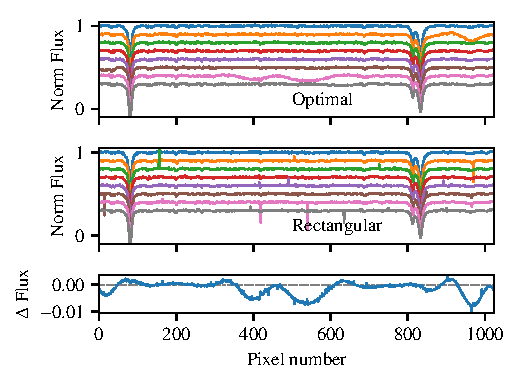
\includegraphics[width=0.7\linewidth]{figures/appendix/bp_plots/extraction_comparision_HD30501-2b_chip_2}
    \caption{Example of DRACS artefacts in the optimally extracted spectra second detector of the second observation of {HD\,30501}.
        top: The 8 normalized nod spectra obtained using \emph{optimal} extraction, vertically offset from each other.
        middle: The 8 normalized nod spectra obtained using \emph{rectangular} extraction, vertically offset from each other.
        bottom: Difference between the combined average spectra from the top and middle panels.
        The middle panel creates the small spikes, while the large deviations are due to the artefacts in the optimal reduction.
        There are four bad pixel spikes that cause artefacts in the optimal extraction.
        These are located in the second nod (orange) around pixel 950, the sixth nod (brown) around pixel 20 and two spikes in the seventh nod (pink) around pixels 400 and 550.}
    \label{fig:artefact_example7}
\end{figure}

%\textbf{
%    EXAMPLE with the new-old \cref{fig:badpixelreplacement}}.
%\todo{CHANGE the figure here}
%\begin{figure}
%    \centering
%    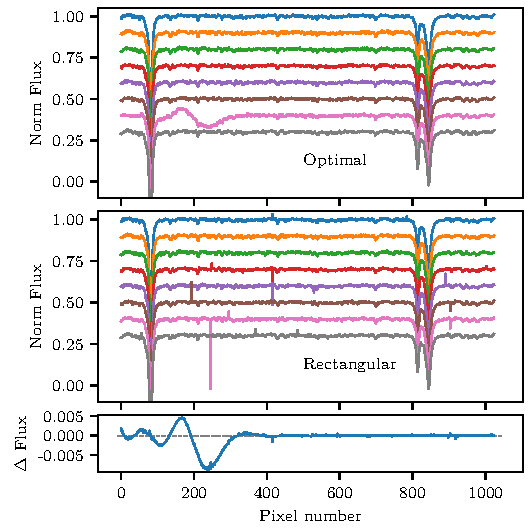
\includegraphics[width=\hsize/2]{figures/reduction/bp_plots/Bad_pixel_replacement}
%    \caption{Example of an artefact in the optimally extracted spectra from detector \#2 of {\red{} HDXXXXXX}.
%        The top panel contains the 8 normalized nod spectra obtained using optimal extraction.
%        The middle panel shows the same nod spectra reduced using only rectangular extraction.
%        The bottom panel shows the difference between a combined spectrum using optimal nods only and a combined spectrum in which the identified nods are replaced with their rectangular counterparts as per \cref{subsubsec:reductionartefacts}.
%        A vertical offset is included between each spectra for clarity.
%        The nod spectra are in observation order from top to bottom.}
%    \label{fig:badpixelreplacement}
%\end{figure}

It is clear that the artefacts in the optimal extraction occur when there is a corresponding ``bad-pixel'' spike\footnote{Their exact origin is unknown but are likely uncorrected bad-pixels or a cosmic ray.
Here they will be referred to as bad-pixels.} in the rectangular extraction.
However this is not always the case with many spikes observed (e.g. third nod around pixel 150 in \cref{fig:artefact_example7}) but automatically removed in the optimal extraction.
The occurrence of artefacts in the observations did not appear to have a pattern with nod position or detector with 14\% (79/544 spectra) of the nod spectra having an optimal exaction that seemed to misbehave.
The artefacts in the optimal extraction are also largely extended, significantly affecting more of the spectrum that the individual spikes (up to 100s of pixels).
Artefacts were observed arising from both large and small spikes alike while other large and small spikes are removed.
This possibly suggests that their size is of less importance, that some other unknown factor (possibly location).

As mentioned in \cref{subsec:extraction} the \emph{optimal} extraction includes variance weighting across the spatial direction.
It appears that the presence of the bad pixel spikes heavily affects the variance weighting procedure during the \emph{optimal} extraction.

Numerous parameters in the {DRACS} pipeline were experimented with in the attempt to remove the observed artefacts with limited success.
For instance, no complete removal of the artefacts was found by adjusting the \(\sigma\) rejection limits (between \(1-5 \sigma\)) or  increasing the tracing width parameter in {IRAF}s DOSLIT\footnote{Documentation for DOSLIT can be found here \href{http://stsdas.stsci.edu/cgi-bin/gethelp.cgi?doslit}{http://stsdas.stsci.edu/cgi-bin/gethelp.cgi?doslit}} recipe, although they did slightly affect the shape of the artefacts.
\cref{fig:resizednods} shows the extraction of HD\,202206 with one parameter changed in the reduction pipeline.
The only difference between the left and right panels the automated aperture resizing\footnote{Using \href{apresize}{http://stsdas.stsci.edu/cgi-bin/gethelp.cgi?apresize.hlp}} was enabled by setting the ``resize'' parameter to \emph{yes} in the right hand panel.
This manages to remove an ugly artefact in the sixth nod (brown), but not the artefact in the seventh nod (pink).
This was only discovered in the writing of this thesis so could not be utilized earlier.
However, it does indicate that some improvements may be obtained with extensive time and patience tweaking the parameters of the {DRACS} pipeline.

\begin{figure}
    \centering
    \begin{tabular}{cc}
        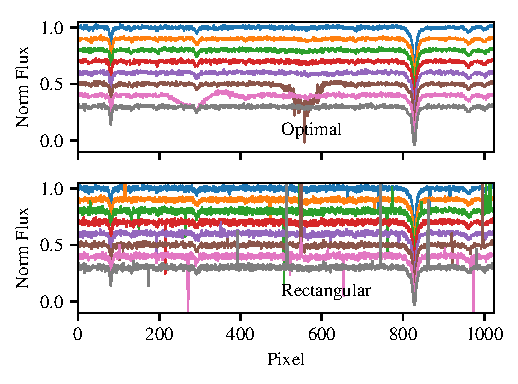
\includegraphics[width=0.5\linewidth]{figures/reduction/bp_plots/non_resized_nods_HD202206-1_chip_2} & 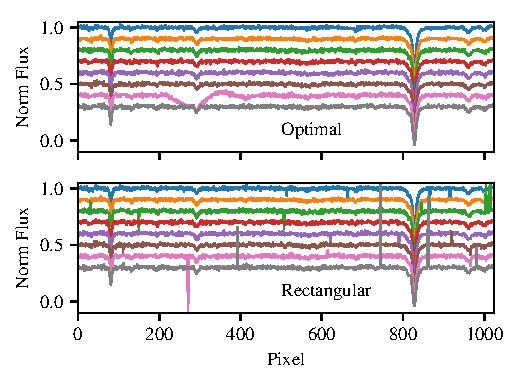
\includegraphics[width=0.5\linewidth]{figures/reduction/bp_plots/resized_nods_HD202206-1_chip_2}\\
    \end{tabular}\label{fig:resizednods}
    \caption{Two {DRACS} reductions for detector \#2 of HD202206-1 with one pipeline parameter changed.
        Left: The reduction with the DRACS pipeline with the ``doslit.resize'' set to ``no''.
        Right: The reduction from the same pipeline but with ``doslit.resize'' set to ``yes'', all else equal.
        During the order tracing the aperture size is automatically adjusted while the rest of the parameters remain identical.
        One large artefact is removed in the sixth nod (brown) while the artefact in the seventh nod (pink) is not removed.}
\end{figure}

The purpose of these observations was to detect faint companion spectra with expected flux ratios \(\rm {F_2}/{F_1} < 1\%\).
As the artefacts created large and extended deviations in the combined spectra (up to 2\%) measures were needed to remove these artefacts from the combined spectra.
To avoid contaminating the spectra of the faint companions.

After the unsuccessful tweaking of parameters the solution that was chosen was to replace the optimally extracted nods that contained artefacts with their rectangular counterparts.
This would create a combined spectra that had a mix of optimally reduced and rectangularly reduced nod spectra, without any artefacts.
To replace the spikes in the rectangular extraction that created the artefacts and others an iterative 4-\(\sigma\)\footnote{There is no scientific justification why 4-\(\sigma\) was chosen over the commonly used 3-\(\sigma\).} rejection algorithm\footnote{Found at \url{https://github.com/jason-neal/nod_combination}} was applied to the rectangular extractions.
The \(\sigma\) for each pixel was calculated as the standard deviation of the nearest 2 pixels on either side of it, across all 8 nod spectra (a $5\times8$ grid).
Any rejected pixels were replaced using linear interpolation along the spectra.
The spectra that contained artefacts and that were replaced using this method are given in \cref{tab:nod_replacement}.

Combined spectra were finally constructed by averaging the eight nod-cycle spectra together, where some of the optimally extracted spectra were replaced using the above method.
The actual spectra from the two different methods can be seen in \cref{fig:reduction-comparison} where orange is the combination of optimally reduced spectra only and green uses the replacement method outlined here.
The easiest to notice a difference is {HD\,202206-1 \#2} in which the artefacts from \cref{fig:resizednods} are removed.

The continuum normalization of the spectra is performed in {IRAF} while the swapping of nods creating a mixed combination is carried out in \emph{Python} along with the post reduction procedures detailed below.

The DRACS pipeline was originally chosen over the {ESO} {CRIRES} pipeline because it seemed relatively simpler to use, being semi-automated, and appeared to have less bad pixel/cosmic ray artefacts in the resulting spectra.
In hindsight the DRACS pipleline had several unexpected challenges due to these artefacts which took time to investigate and find a solution for.

One hypothesis for these artefacts is detector glow, the heating of the detector by the nearby amplifiers in the chip (see \cref{subsubsec:darkcurrent}.
The artefacts in the \emph{K}-band spectra were not observed in previous works in the \emph{H}-band using this pipeline~\citep[e.g.][]{figueira_radial_2010}, and as such may have a wavelength dependent effect, like detector glow.
However, it seems plausible that a glow related effect would be spatial distributed like the glow shown in \cref{fig:darkcurrent_colour}, but the location of the artefacts do not seem to have a discernible pattern.
It could also be that there were artefacts in intermediate steps of the previous works that were missed due to the semi-automated pipeline, with the resultant combined spectrum being only slightly affected at the level of >1\% it could easily be missed (e.g. \cref{fig:reduction-comparison}).
Anther possibility is that the artefacts are bad pixels not removed correctly.
Regardless, in the end they do not have a significant impact on the results found in this work, though it is expected that mixing the optimal and rectangular extracted spectra will have a slight negative impact on the noise or \snr{} of the combined spectrum.
Much time and effort was invested attempting to extract the spectra, without artefacts, to have the best chance at obtaining high quality scientific results of the faint features sought after in this work.
